\section{$k$-ary Trees}\label{s:k-ary_trees}
When analyzing a general problem of graph drawings, considering trees may come in handy due to their assessable properties. The first graph class considered for minimizing the ratio in a drawing is therefore the class of $k$-ary trees. This section describes a drawing algorithm for a $k$-ary tree $T$, guaranteeing a nearly optimal euclidian ratio in the resulting drawing $\Gamma_T$. The total area of $\Gamma_T$ will depend on the height of $T$.\\
% properties of complete k-ary trees
Since any $k$-ary tree is acyclic per definition, $T$ is connected, but not biconnected and the treewidth of $T$ equals 1. Having $n$ vertices, $T$ inherits exactly $n-1$ edges. The small bags in a tree decomposition and the low amount of edges makes $k$-ary trees accessible for a straightforward solution for a given problem.\\
% context for outerplanar graphs
When working on other graph classes, it may be possible to find an approach by reducing a graph $G$ to an instance of a tree. In fact, this effect will occur in the subsequent section of this thesis.
\subsection{Properties Of Complete $k$-ary Trees}
% The height 
\begin{lemma}The \emph{height $h$} of a complete $k$-ary tree $T$ is in $\mathcal{O}(\log n)$.\label{l:k-ary-tree_log_height}
\end{lemma}
\begin{proof}
	\begin{align}
		n = \sum_{i=0}^{h}k^i &= \frac{k^{h+1}-1}{k-1}\\
		\Leftrightarrow h &= \log_k((k-1)n+1)-1\\
		&= \frac{\log((k-1)n+1)}{\log k}-1\\
		\underbrace{\Rightarrow}_{k \text{ constant}}h &\in O(\log n)
	\end{align}
\end{proof}

\subsection{The Drawing Algorithm}

% Drawing result

\begin{theorem}
	Every complete $k$-ary tree admits a planar straight-line drawing with a nearly optimal ratio, apart from a rounding error, on area $\mathcal{O}(n^2\log n)$.
\end{theorem}
\begin{proof}
	The following drawing will be constructed from top to bottom, meaning that the $y$-coordinates of the children of any vertex $v$ are smaller than the $y$ coordinate of $v$.\\
	Let $r := k^h$. For a vertex $v$ in height $i$, consider $k$ equidistant columns with $x$-coordinates between $x(v) - (k-1)\cdot  k^{h-h'-1}$ and $x(v) + (k-1)\cdot  k^{h-h'-1}$. These are integer coordinates since the distance between two columns next to each other equals $2\cdot \frac{k^{h-i}}{k}$. Draw a circle around $v$ with radius $r$. Choose the grid points $v_i$ on the column closest to the resulting intersections with the constraint that $y(v_i) \leq y(v)$ and connect $v$ with its $k$ children with a straight-line.
	% TODO Illustration of circle with columns
\begin{figure}[H]
	\centering
		\begin{subfigure}{\textwidth}
			\centering
			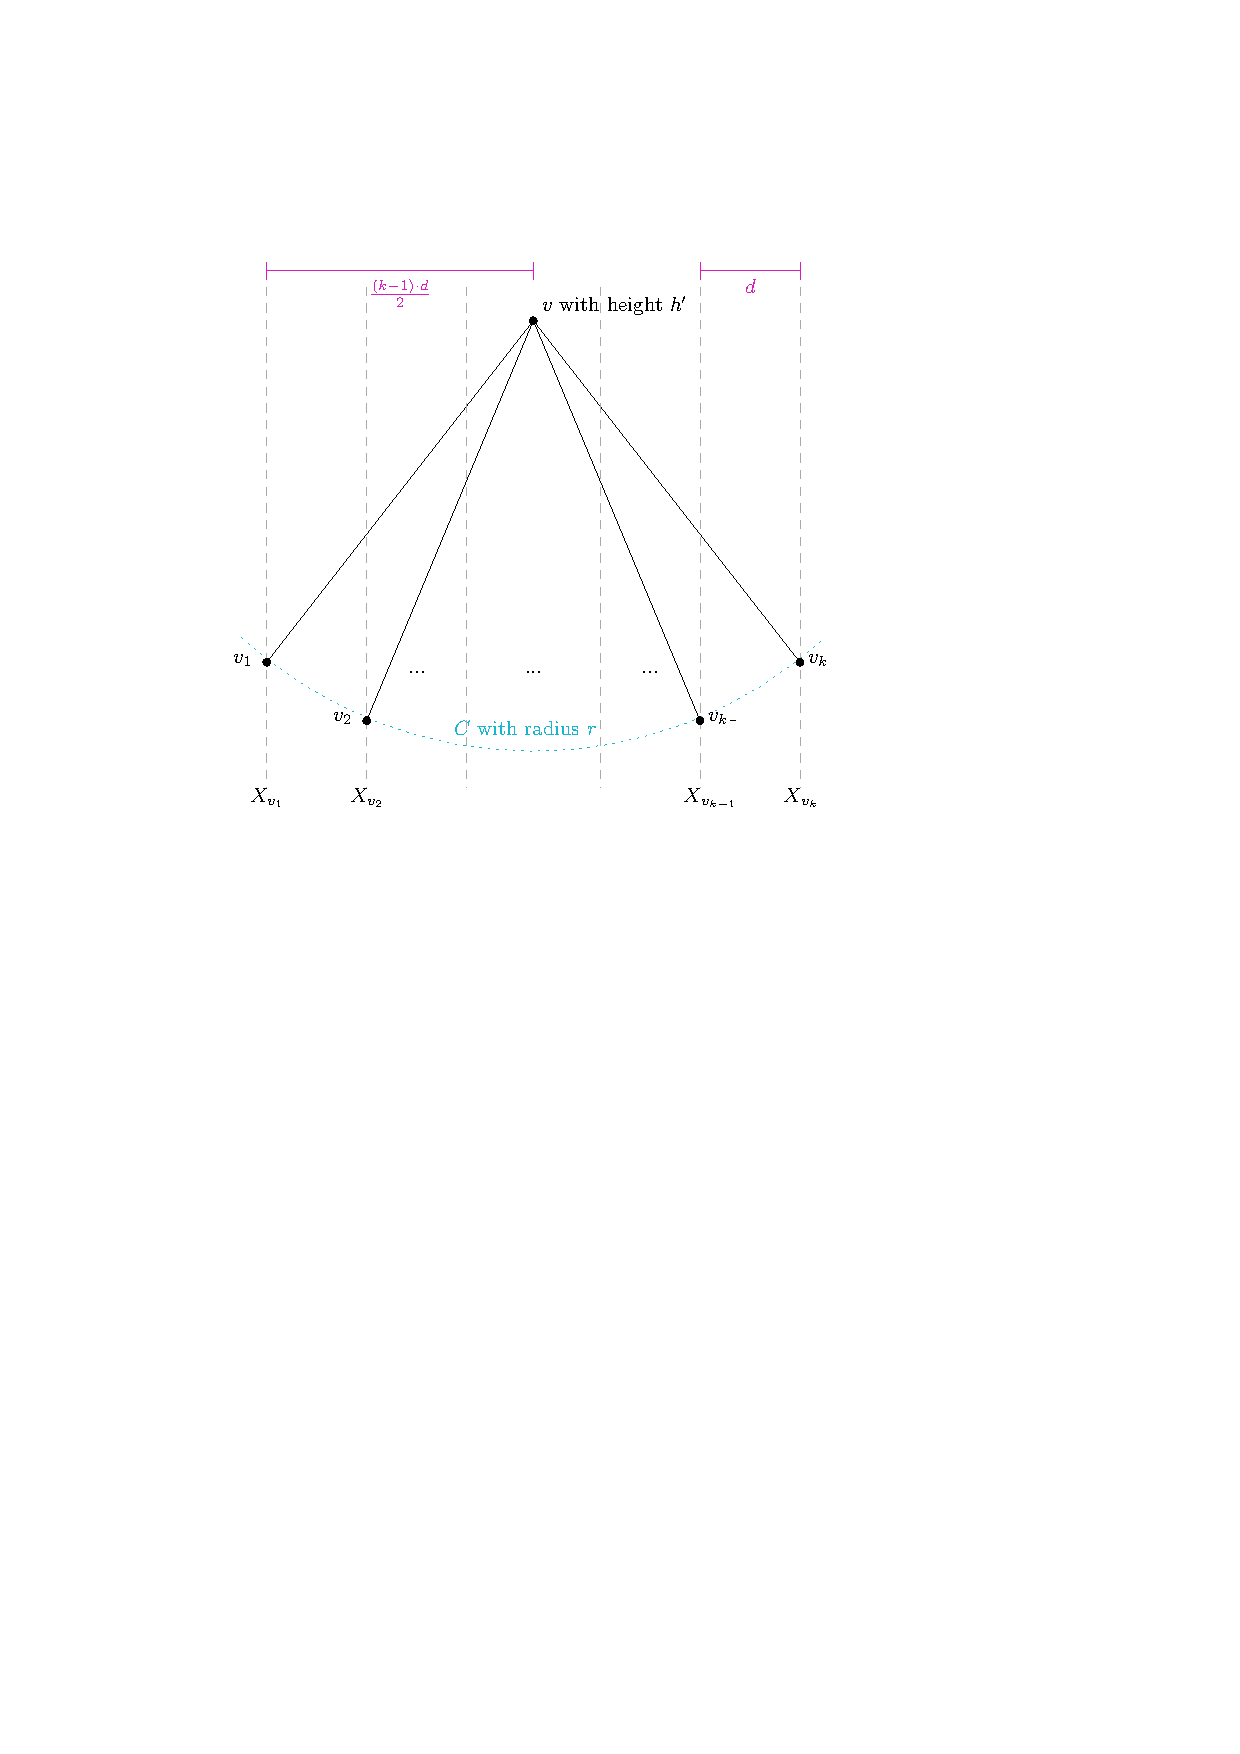
\includegraphics[page=1,width=0.8\linewidth]{graphics/k-ary_tree_algorithm_construction.pdf}
		\end{subfigure}
	\caption{Illustration of drawing algorithm at a vertex $v$ with height $h$}\label{im:k-ary_trees_algorithm_illustration}
\end{figure}
	The distance between two neighbouring columns in height $i$ suffices for the remaining drawing since it holds for the remaining heights:
	\begin{align}
		\underbrace{2\cdot \sum_{j=i}^{h-1} k^{h-j-1}}_{\text{drawn from both columns}} &= 2\cdot\sum_{z = 0}^{h-i-1}h^z\\
		&= 2\cdot\frac{k^{h-i}-1}{k-1} < 2\cdot k^{h-i}
	\end{align}
	The height of the drawing is bound by $h\cdot r = h\cdot k^h \in \mathcal{O}(n\cdot \log n)$. 
	The width is bound by $2\cdot\sum_{i = 0}^{h} k^i = 2\cdot \frac{k^{h+1}-1}{k-1} \in \mathcal{O}(n)$, resulting in $\mathcal{O}(n^2\log n)$ area.\\ 
	Since the algorithm works from top to bottom and for height $i$, the area for every subtree is disjointedly reserved, the resulting drawing is planar. Furthermore, all straight-line edges inherit a length of approximately $k^h$, no bends were used and the ratio is bound by $1+\varepsilon, 0\leq \varepsilon<1$.
\end{proof}
\bigskip
The following algorithm sums up the approach described above.\\
\begin{algorithm}[H]
	\KwIn{complete $k$-ary tree $T$, $h$}
	\KwOut{Straight-line drawing of $T$ with nearly optimal ratio}
	\caption{Draw\_$k$-ary\_tree($h$)}\label{al:complete_k-ary_tree}
	$h \gets $ \text{height of $T$}\\
	$r \gets k^h$\\
	Draw $root(T)$ on any grid point\\
	\texttt{Draw\_$k$-ary\_Children}$(root(T),r,h)$\\
	\Return $\Gamma$
\end{algorithm}
\begin{algorithm}[H]
	\KwIn{Already drawn vertex $v$, radius and height $r,h \in \mathbb{N}$}
	\KwOut{Coordinates of all the children of $v$}
	\caption{\texttt{Draw\_$k$-ary\_Children}$(v,r,h)$}
	\If{$v$ leaf}{\Return}
	\Else{
		$h' \gets \texttt{height}(v)$\\
		$d \gets 2\cdot k^{h-h'-1}$\\
		$C \gets \Gamma.\texttt{DrawCircle}(r,v)$\\
		\tcc{Draw circle with radius $r$ around $v$}
		\For{$i \in [1..k]$}{
			$x(v_i) \gets x(v) - \frac{(k-1)\cdot d}{2} + (i-1)\cdot d$\\
			\tcc{$x$-coordinate of $i$-th child of $v$}
			$X \gets \Gamma.\texttt{Column}(x(v_i))$\\
			\tcc{Identify the column at position $x(v_i)$}
			$s \gets \Gamma.\texttt{Intersection}(I,X)$\\
			\tcc{Calculate the intersection of the circle $C$ and the column $X$}
			$y(v_i) \gets round(y(s))$\\
			$\Gamma.$\texttt{DrawStraightLine}$(v,v_i)$\\
			$\Gamma.$\texttt{Draw\_$k$-ary\_Children}$(v_i,r,h)$
		}
	}		
\end{algorithm}


\subsection{Example Drawings}
% TODO Example drawings
\begin{figure}[H]
	\centering
	\begin{subfigure}{\textwidth}
		\centering
		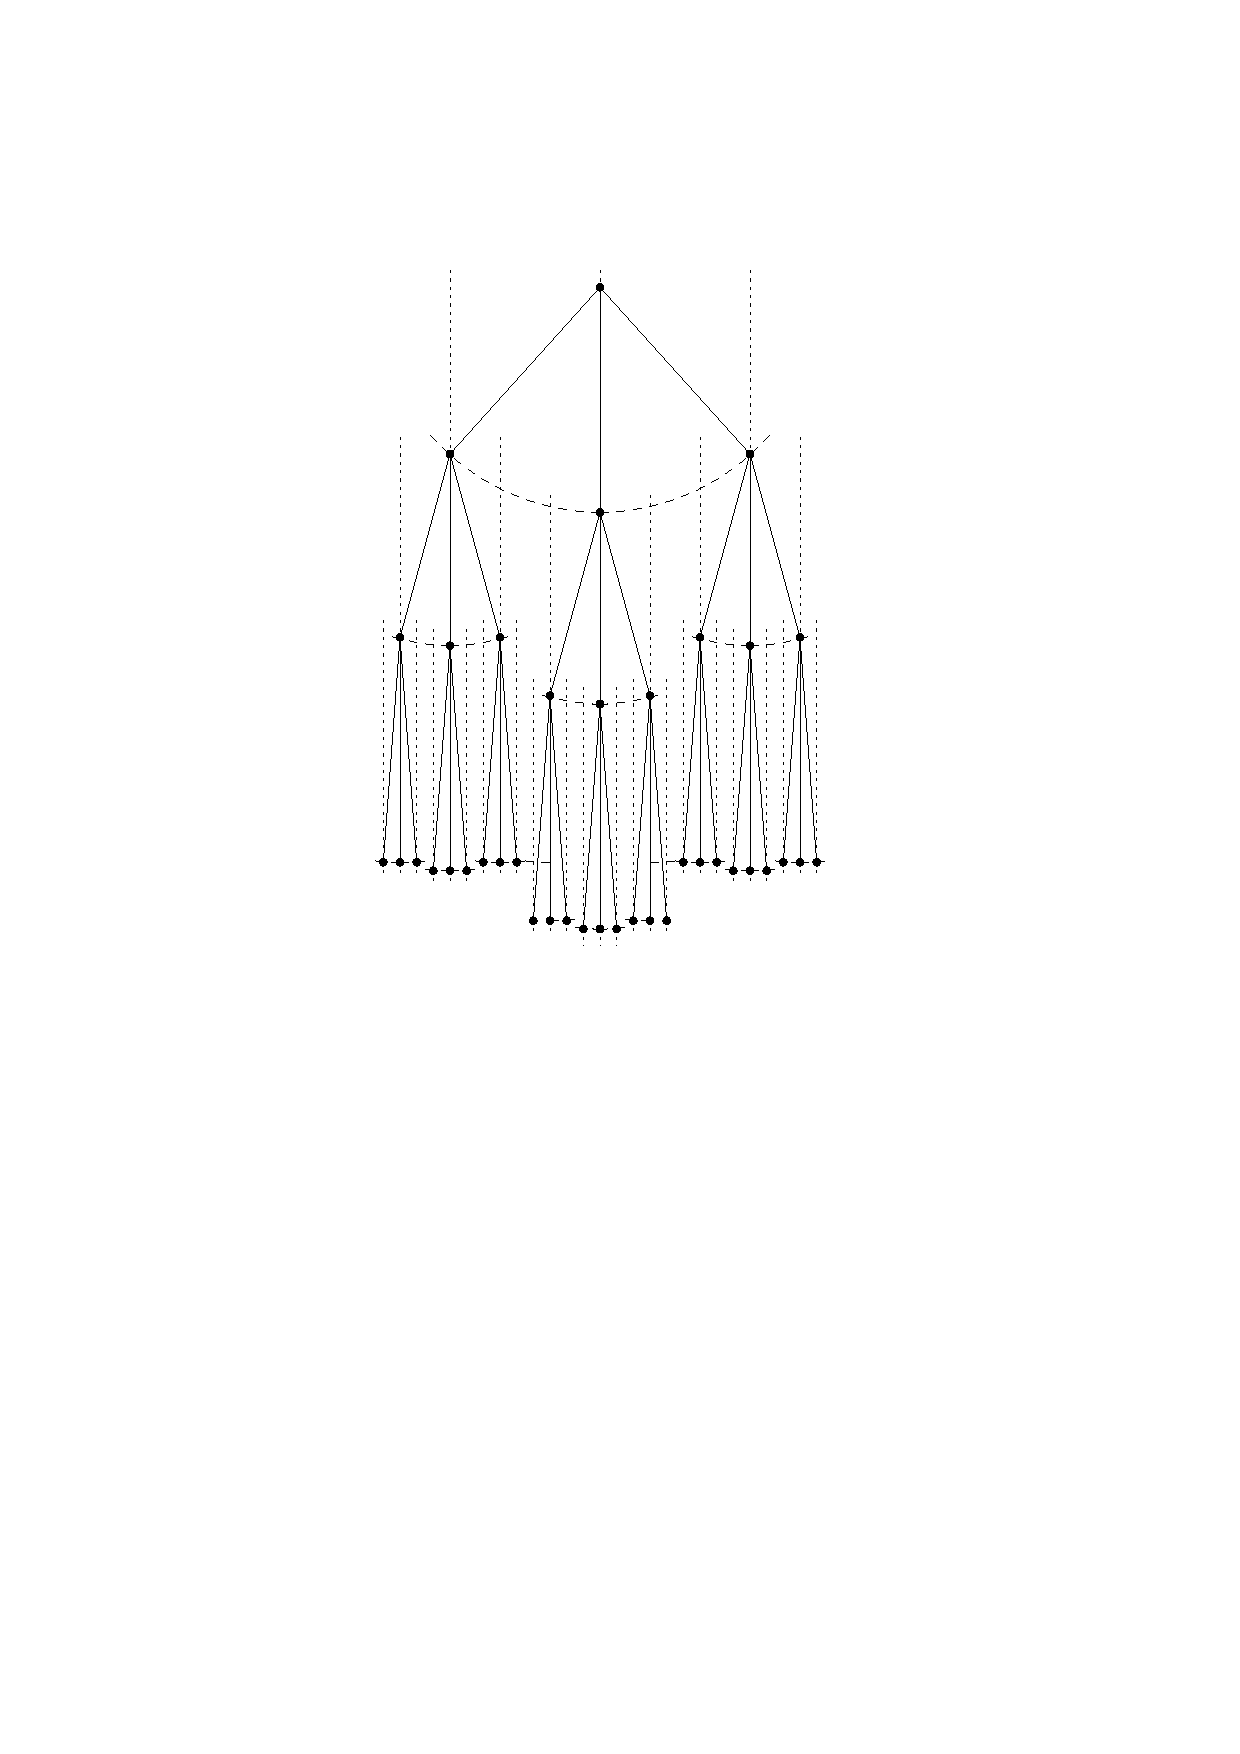
\includegraphics[page=1,width=0.8\linewidth]{graphics/k-ary_tree_example_drawings.pdf}
	\end{subfigure}
	\caption{Tertiary tree with height 3}\label{im:3-ary_tree}
\end{figure}
\begin{figure}[H]
	\centering
	\begin{subfigure}{\textwidth}
		\centering
		\includegraphics[page=2,width=0.8\linewidth]{graphics/k-ary_tree_example_drawings.pdf}
	\end{subfigure}
	\caption{5-ary tree with height 2}\label{im:4-ary_tree}
\end{figure}


\subsection{Partitioning A Binary Tree In Complete Binary Subtrees}

Algorithm \ref{al:complete_k-ary_tree} works fine for complete $k$-ary trees. As a next step, the drawing approach is used when drawing any given $k$-ary tree. 
\begin{lemma}
	The \emph{height $h$} of any $k$-ary tree is in $\Omega(\log n)$ and $\mathcal{O}(n)$.
\end{lemma}
Let $T$ be a chain of vertices with the degree of the root valuing 1, describing the worst case with height $n-1$. One approach would be to extend $T$ to a complete binary supertree $T'$, draw it with algorithm \ref{al:complete_k-ary_tree} and reduce it to $T$ again. This would work in order to produce a nearly optimal drawing on one hand, but, on the other hand, this will explode the area exponentially since with a linear height, the extension from $T$ to $T'$ will insert exponentially many vertices.\\
In order to overcome this issue of exponential area, a partitioning of any given $k$-tree $T$ into complete subtree components will prove being helpful. In fact, partitioning a binary tree will be helpful in further aspects of this thesis.
% TODO figure partition
\begin{definition}
	A \emph{partition} $T_i$ of $T$ is a family of trees with the following properties:
	\begin{itemize}
		\item $\bigcup_{i} V(T_i) = V(T)$
		\item $\bigcup_{i} E(T_i) \subseteq E(T)$
	\end{itemize}
	A partition $T_i$ is \emph{minimal} if for every other partition $T'_j$ of $T$ it holds that $i\leq j$.
\end{definition}
Let $T$ be a $k$-ary tree with $n$ vertices. Then, for a partition $T_i$, the following holds:
\begin{itemize}
	\item The amount of partitions of size $\mathcal{O}(1)$ lies in $\mathcal{O}(n)$
	\item The amount of partitions of size $\mathcal{O}(\log n)$ is bound by $\mathcal{O}\left(\frac{n}{\log n}\right)$
	\item The amount of partitions of size $\mathcal{O}(\sqrt{n})$ is bound by $\mathcal{O}(\sqrt{n})$
	\item The amount of partitions of size $\mathcal{O}(n)$ is bound by a constant
\end{itemize}
  

\begin{theorem}
	Every $k$-ary tree with height $h$ admits a planar straight-line drawing with a nearly optimal ratio, apart from a rounding error, on area $\mathcal{O}(n^2\log n)$.
\end{theorem}
\begin{proof}
	Let $T$ be any rooted $k$-ary tree with height $h$. 
\end{proof}
